
\documentclass[a4paper,12pt]{article}
\usepackage[latin1]{inputenc}
\usepackage[spanish,es-nodecimaldot]{babel}
\usepackage[T1]{fontenc}
\usepackage[intlimits]{amsmath}
\usepackage{graphicx}
\usepackage{a4wide}
\usepackage{float}

\usepackage{tikz}
\usetikzlibrary{trees}
\usepackage{xcolor}

\graphicspath{{imagenes/}}

\title{\textsc{Modelo de Ising en 2D} \\ \vspace{2em} \Large{Introducci�n a la 
simulaci�n computacional}}
\author{\small{Luis Pizarro (lpizarro@cnea.gov.ar)} \\
        \small{Pablo Bellino (pbellino@gmail.com)}}

\date{Octubre de 2015}


\begin{document}
\maketitle

\begin{abstract}
Un resumen
\end{abstract}


\section{Introducci�n}
Empezamo

\tikzstyle{every node}=[thick,anchor=west, 
font={\scriptsize\ttfamily}, inner sep=2.5pt]
\tikzstyle{selected}=[draw=blue,fill=blue!10]
\tikzstyle{root}=[draw=blue, fill=blue!30]

\begin{figure}[H]
\begin{center}
\begin{tikzpicture}[%
    scale=.7,
    grow via three points={one child at (0.5,-0.65) and
    two children at (0.5,-0.65) and (0.5,-1.2)},
    edge from parent path={(\tikzparentnode.south) |- (\tikzchildnode.west)}]
  	\node [root] {bin}
  	child { node [red] {ising}}
  	child { node [red] {corridas\_paralelo.py}}
  	child { node {tablas\_temperatura.dat}}
    child { node [selected] {0.5\_tmpfolder}
      child { node {parametros.dat}}
      child { node {runs\_estadistica.dat}}
      child { node [selected] {RUN00}
	     child { node {val\_medios.dat}}
	     child { node {estado.dat}}
	     child { node {ultimo\_estado.dat}}
      }
      child { node at(0,-1.8) [selected] {RUN01}}
      child { node at(0,-1.9) [selected] {RUN02}}
      child { node at (0,-2.0) {\dots}}
    }       
    child { node at (0,-5.5) [selected]{0.6\_tmpfolder}}
    child { node at (0,-5.8)[selected] {0.7\_tmpfolder}}
    child { node at (0,-6.1) {\dots}};
\end{tikzpicture}
\end{center}
\end{figure}]


%\begin{eqnarray}
%  f_r(x) &=& \frac{4}{\pi - 4}\frac{x^2}{1+x^2} \\
%  f_\theta(x) &=& \frac{\sin(x)}{2} \\
%  f_\varphi(x) &=&  \frac{1}{2\pi} 
%\end{eqnarray}

\begin{figure}[H]
    \begin{center}
      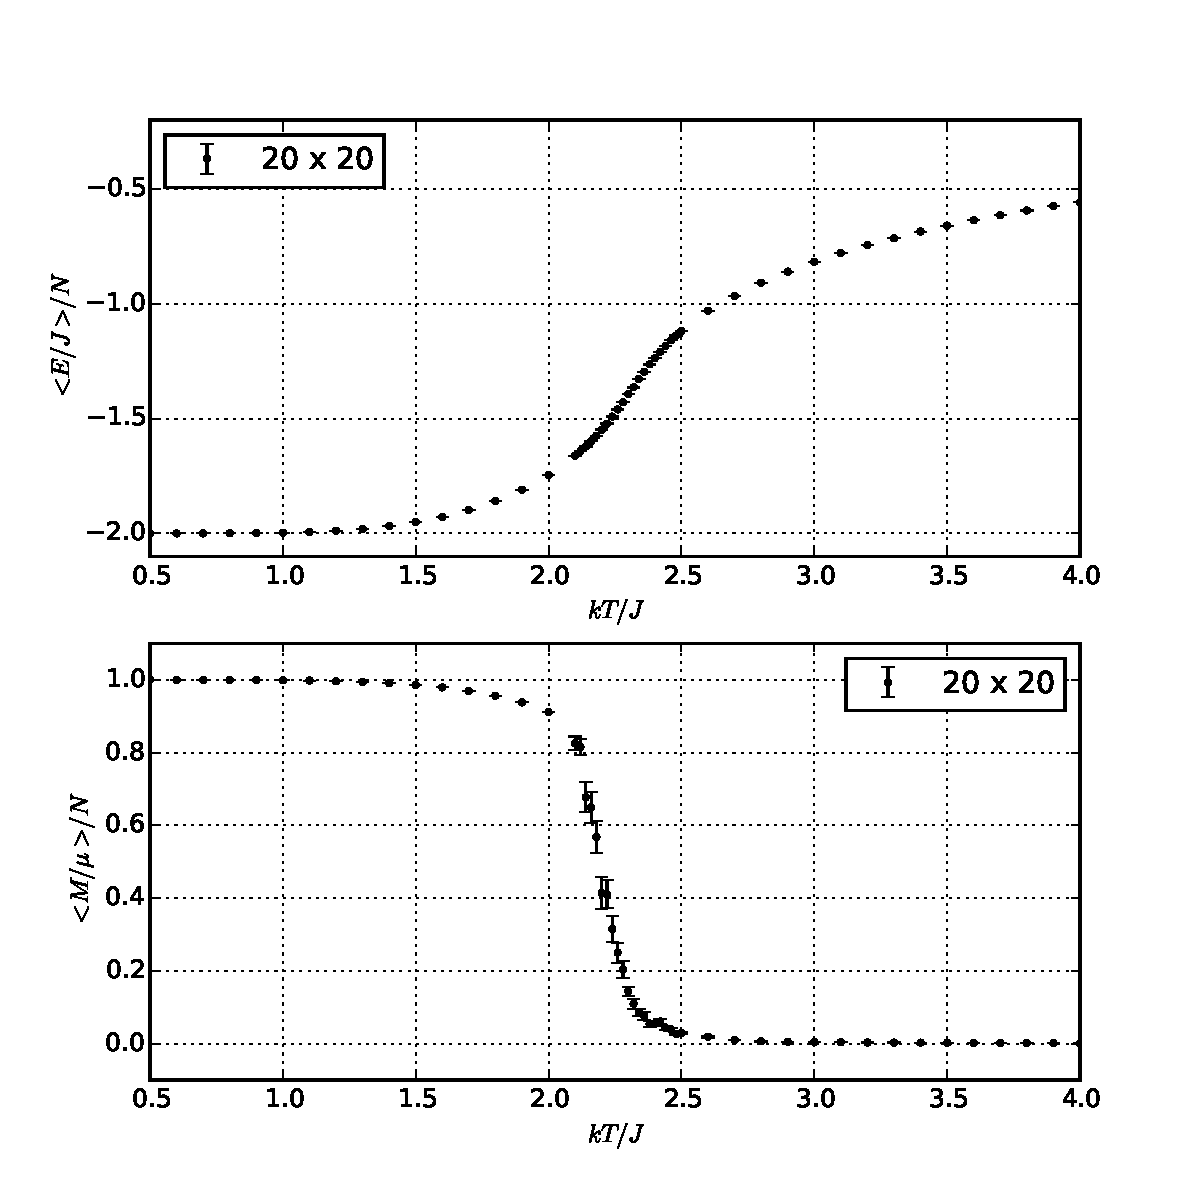
\includegraphics[scale=0.6]{val_medios.pdf} \\
      \caption{Distribuci�n poissonianas $P(4)$, $P(10)$ y $P(40)$. En rojo 
      aparecen las distribucciones gaussianas para cada 
      caso.}\label{fig:val_medios}
    \end{center}
\end{figure}


\begin{figure}[H]
    \begin{center}
      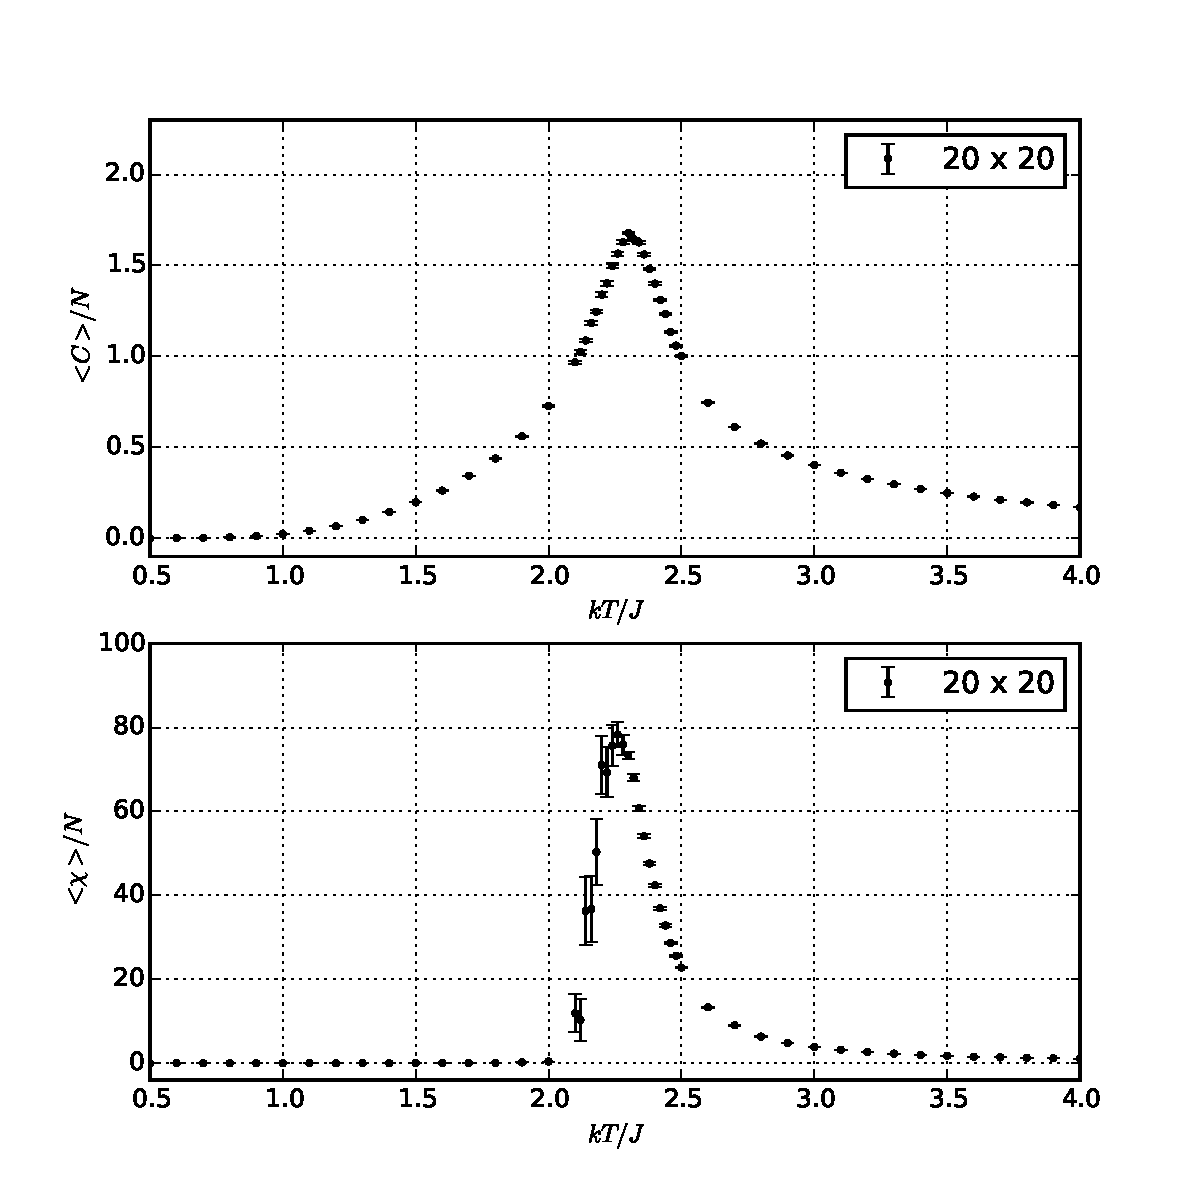
\includegraphics[scale=0.6]{fluctuaciones.pdf} \\
      \caption{Distribuci�n poissonianas $P(4)$, $P(10)$ y $P(40)$. En rojo 
      aparecen las distribucciones gaussianas para cada 
      caso.}\label{fig:fluctuaciones}
    \end{center}
\end{figure}

\begin{figure}[H]
    \begin{center}
      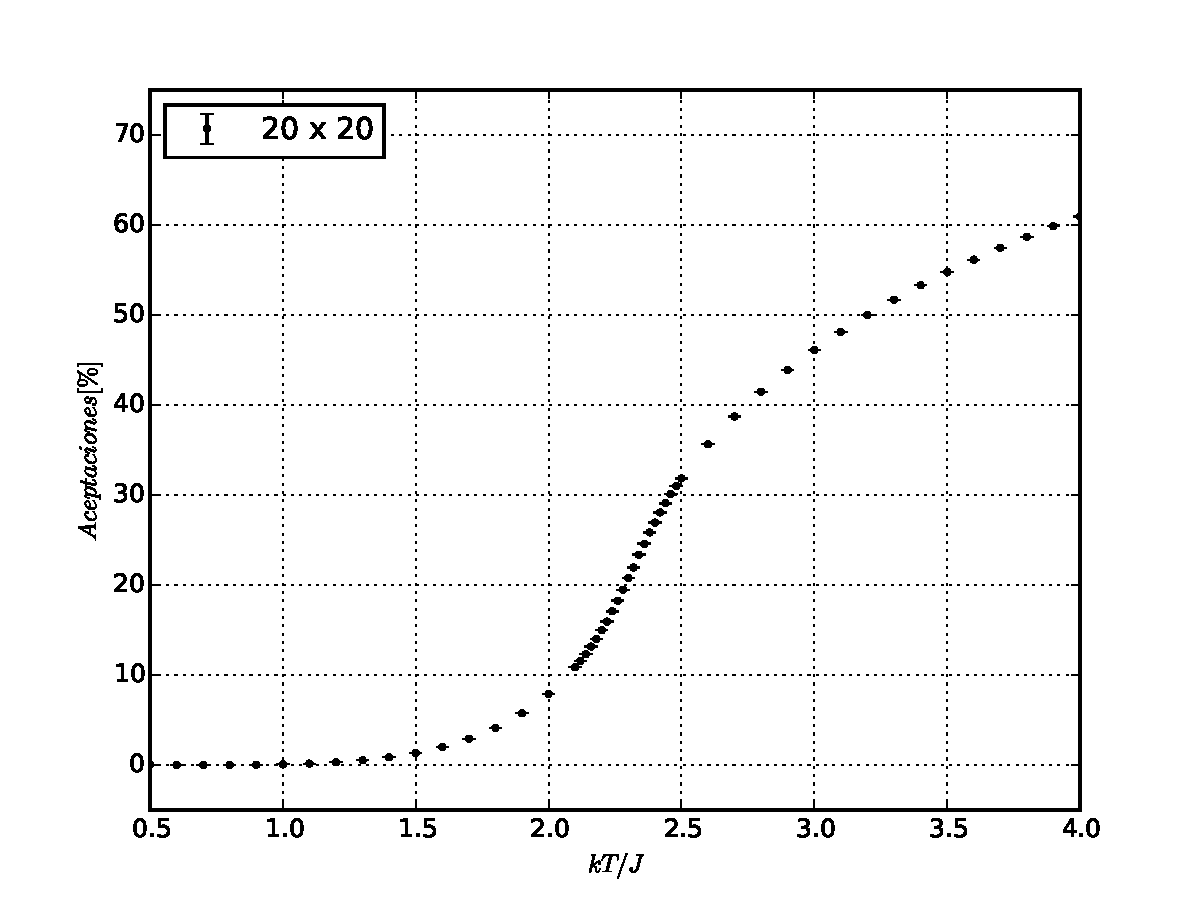
\includegraphics[scale=0.5]{aceptaciones.pdf} \\
      \caption{Distribuci�n poissonianas $P(4)$, $P(10)$ y $P(40)$. En rojo 
      aparecen las distribucciones gaussianas para cada 
      caso.}\label{fig:aceptaciones}
    \end{center}
\end{figure}


\begin{figure}[H]
    \begin{center}
      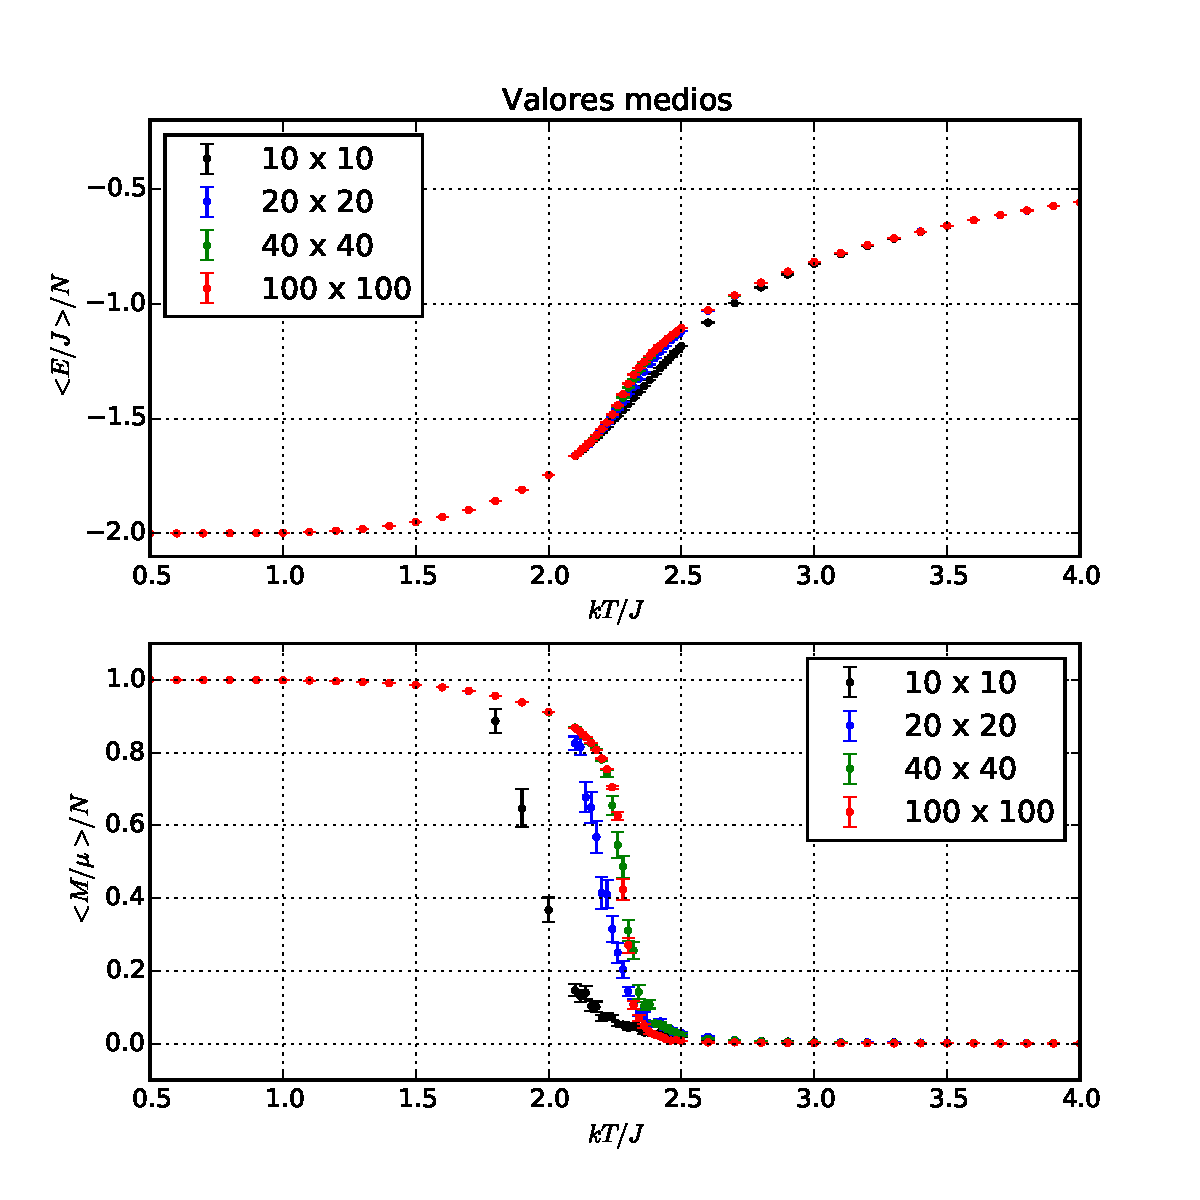
\includegraphics[scale=0.6]{tamano_val_medios.pdf} \\
      \caption{Distribuci�n poissonianas $P(4)$, $P(10)$ y $P(40)$. En rojo 
      aparecen las distribucciones gaussianas para cada 
      caso.}\label{fig:tam_val_medios}
    \end{center}
\end{figure}

\begin{figure}[H]
    \begin{center}
      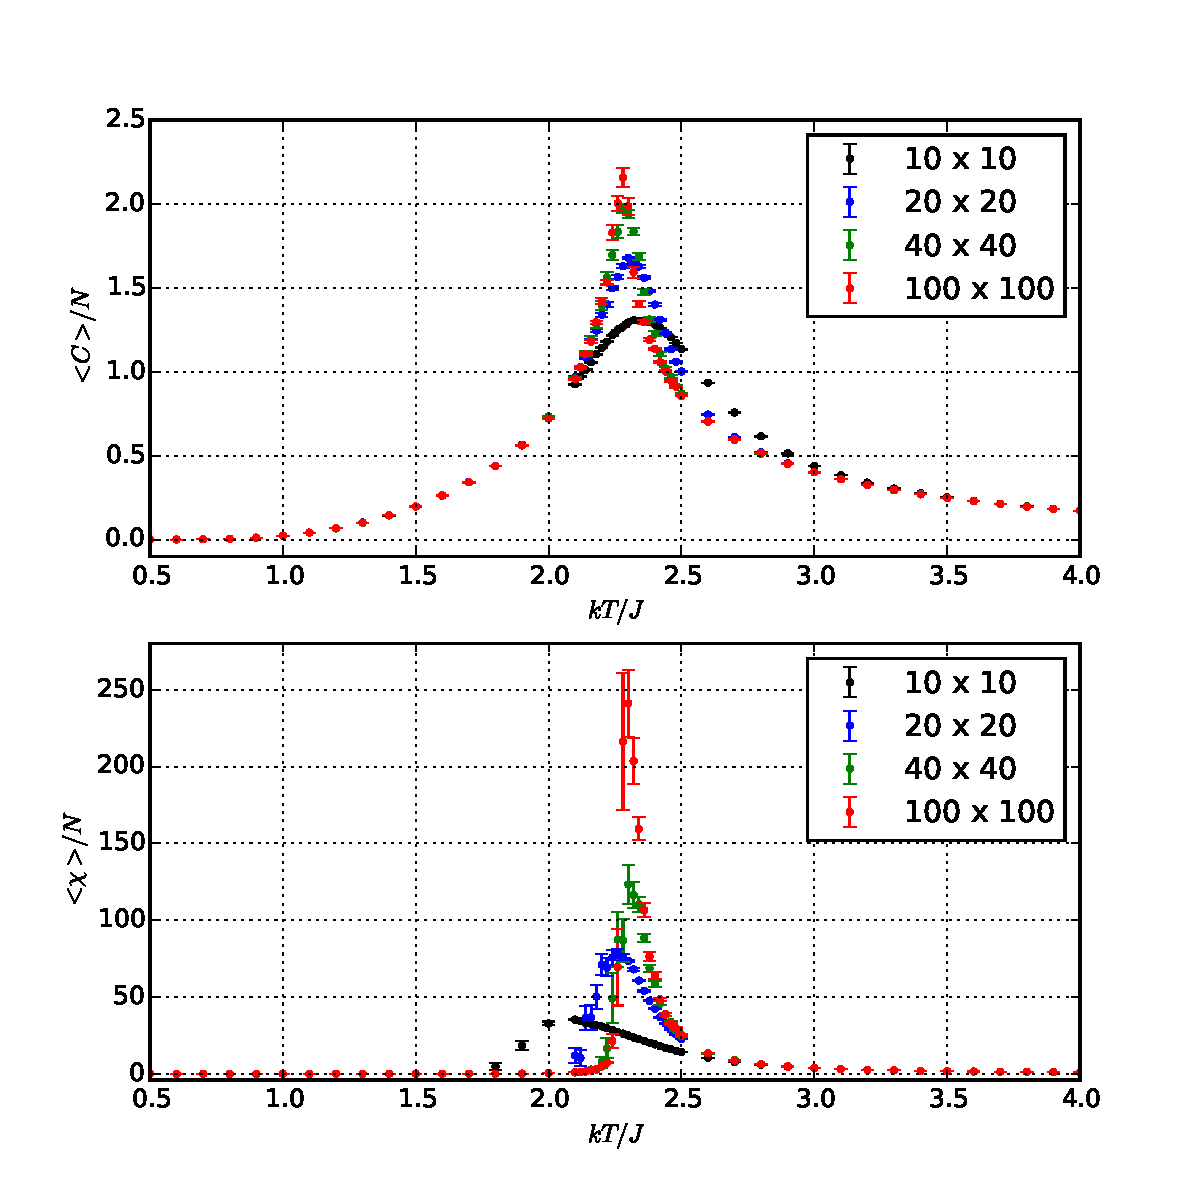
\includegraphics[scale=0.6]{tamano_fluctuaciones.pdf} \\
      \caption{Distribuci�n poissonianas $P(4)$, $P(10)$ y $P(40)$. En rojo 
      aparecen las distribucciones gaussianas para cada 
      caso.}\label{fig:fluctuaciones}
    \end{center}
\end{figure}

\begin{figure}[H]
    \begin{center}
      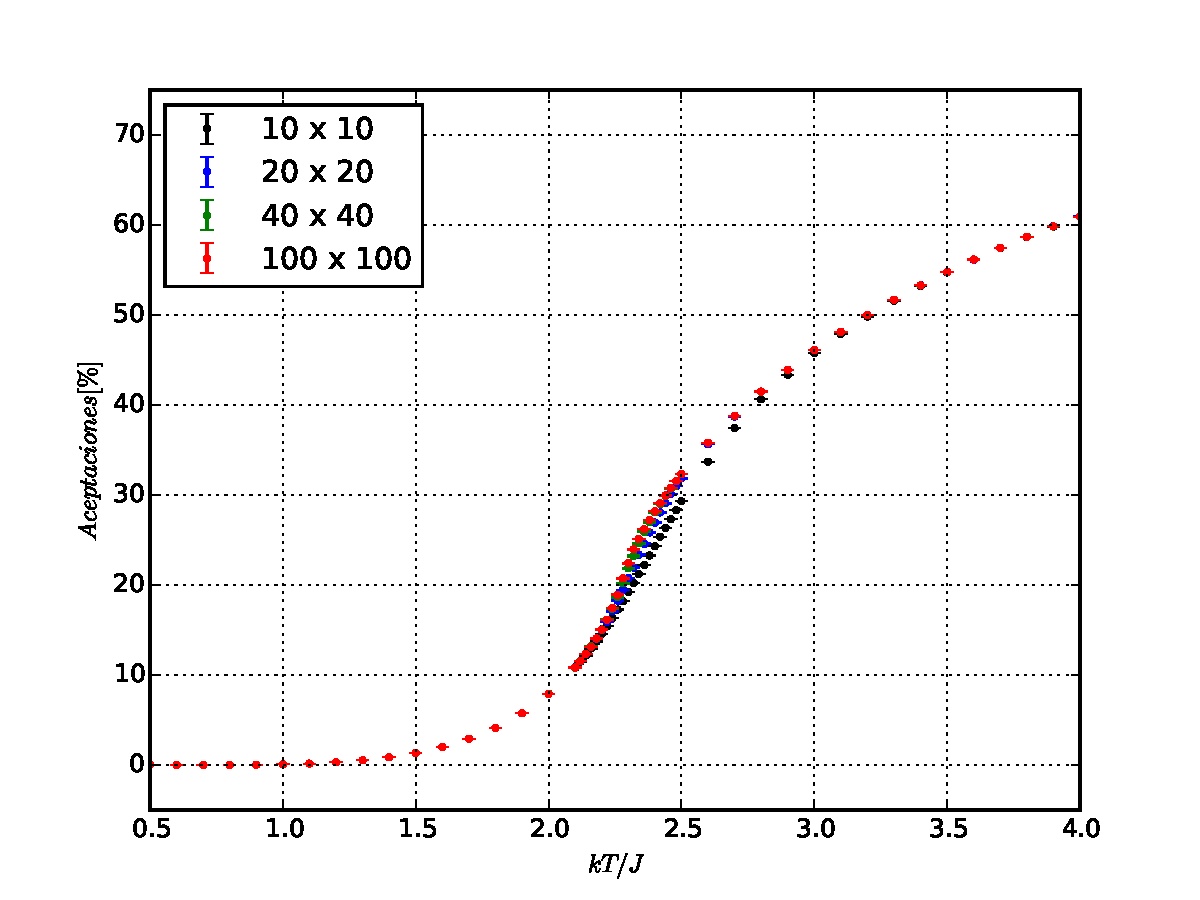
\includegraphics[scale=0.5]{tamano_aceptaciones.pdf} \\
      \caption{Distribuci�n poissonianas $P(4)$, $P(10)$ y $P(40)$. En rojo 
      aparecen las distribucciones gaussianas para cada 
      caso.}\label{fig:aceptaciones}
    \end{center}
\end{figure}

\begin{figure}[H]
    \begin{center}
      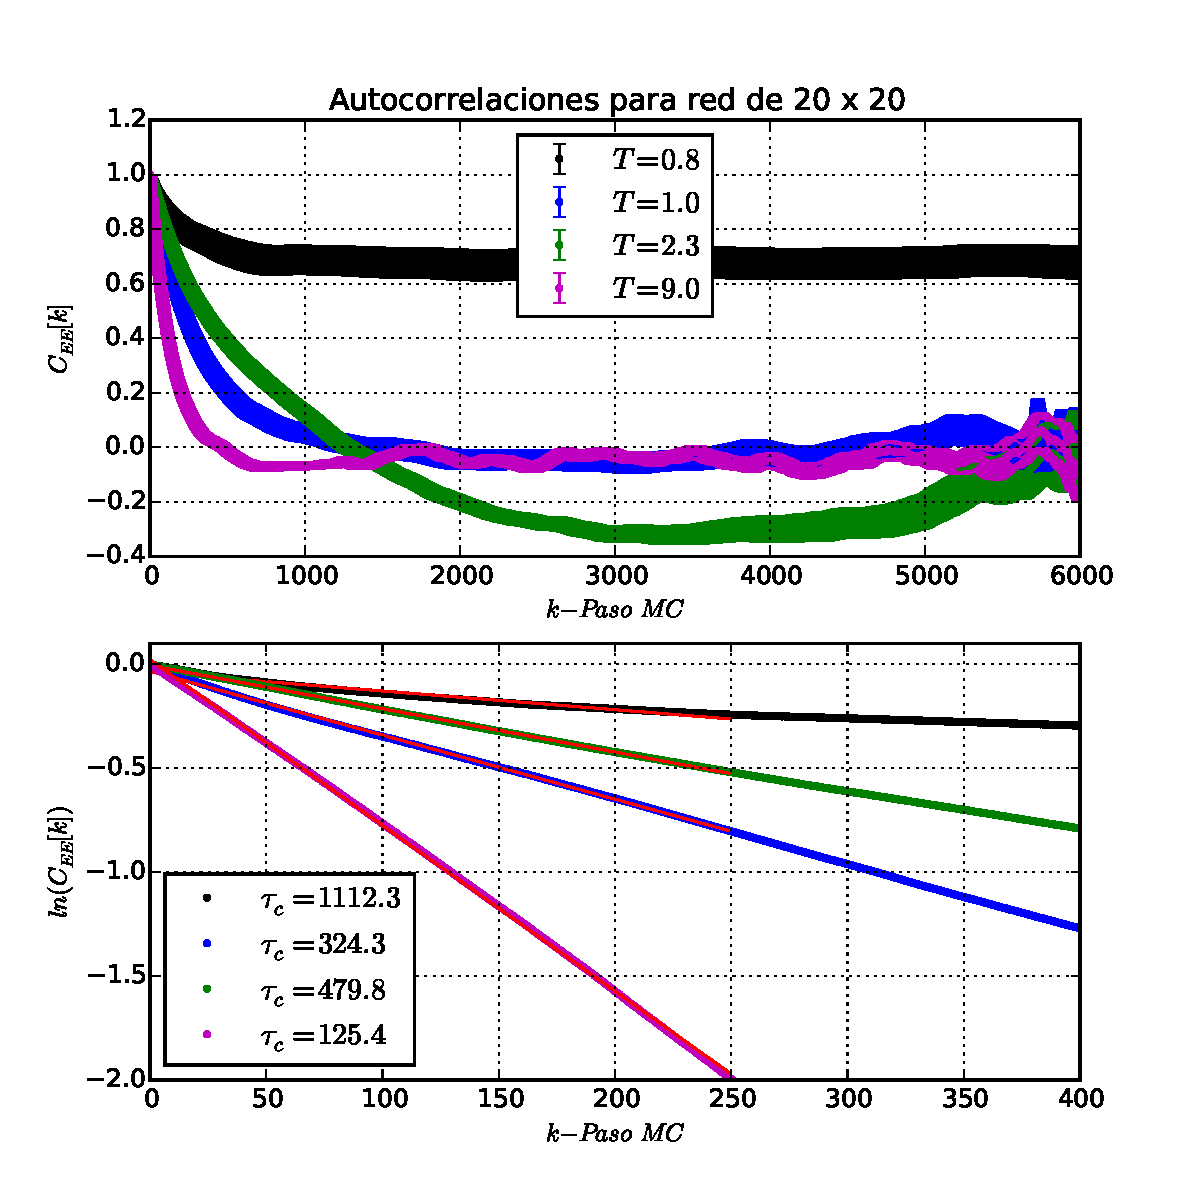
\includegraphics[scale=0.5]{corre_20x20.pdf} \\
      \caption{Distribuci�n poissonianas $P(4)$, $P(10)$ y $P(40)$. En rojo 
      aparecen las distribucciones gaussianas para cada 
      caso.}\label{fig:corre_20x20}
    \end{center}
\end{figure}

\begin{figure}[H]
    \begin{center}
      \includegraphics[scale=0.5]{{corre_tamano_t2.3}.pdf} \\
      \caption{Distribuci�n poissonianas $P(4)$, $P(10)$ y $P(40)$. En rojo 
      aparecen las distribucciones gaussianas para cada 
      caso.}\label{fig:corre_tamano_t2}
    \end{center}
\end{figure}

\begin{figure}[H]
    \begin{center}
      \includegraphics[scale=0.5]{{corre_tamano_t9.0}.pdf} \\
      \caption{Distribuci�n poissonianas $P(4)$, $P(10)$ y $P(40)$. En rojo 
      aparecen las distribucciones gaussianas para cada 
      caso.}\label{fig:corre_tamano_t9}
    \end{center}
\end{figure}

\begin{figure}[H]
    \begin{center}
      \includegraphics[scale=0.5]{{corre_tamano_t9.0}.pdf} \\
      \caption{Distribuci�n poissonianas $P(4)$, $P(10)$ y $P(40)$. En rojo 
      aparecen las distribucciones gaussianas para cada 
      caso.}\label{fig:corre_tamano_t9}
    \end{center}
\end{figure}

\section {Evoluci�n de la matriz de estado de spines en funci�n de la temperatura}


Para las temperaturas

\begin{figure}[ht]
	\begin{minipage}[b]{0.45\linewidth}
		\centering
		\includegraphics[width=\textwidth]{{frame5.0}.pdf}
		\caption{Temperatura 5.0}
		\label{fig:temperatura5.0}
	\end{minipage}
	\hspace{0.5cm}
	\begin{minipage}[b]{0.45\linewidth}
		\centering
		\includegraphics[width=\textwidth]{{frame3.8}.pdf}
		\caption{Temperatura 3.8}
		\label{fig:temperatura3.8}
	\end{minipage}
\end{figure}

\begin{figure}[ht]
	\begin{minipage}[b]{0.45\linewidth}
		\centering
		\includegraphics[width=\textwidth]{{frame2.3}.pdf}
		\caption{Temperatura 2.3}
		\label{fig:temperatura2.3}
	\end{minipage}
	\hspace{0.5cm}
	\begin{minipage}[b]{0.45\linewidth}
		\centering
		\includegraphics[width=\textwidth]{{frame2.0}.pdf}
		\caption{Temperatura 2.0}
		\label{fig:temperatura2.0}
	\end{minipage}
\end{figure}


\begin{figure}[ht]
	\begin{minipage}[b]{0.45\linewidth}
		\centering
		\includegraphics[width=\textwidth]{{frame1.3}.pdf}
		\caption{Temperatura 1.3}
		\label{fig:temperatura1.3}
	\end{minipage}
	\hspace{0.5cm}
	\begin{minipage}[b]{0.45\linewidth}
		\centering
		\includegraphics[width=\textwidth]{{frame0.5}.pdf}
		\caption{Temperatura 0.5}
		\label{fig:temperatura0.5}
	\end{minipage}
\end{figure}

\end{document}
